\documentclass[11pt,a4paper]{article}

\usepackage[margin=2.2cm]{geometry}
\usepackage[T1]{fontenc}
\usepackage{lmodern}
\usepackage{microtype}
\usepackage{graphicx}
\usepackage{booktabs}
\usepackage{tabularx}
\usepackage{xltabular}
\usepackage{array}
\usepackage{xcolor}
\usepackage{listings}
\usepackage{enumitem}
\usepackage{caption}
\usepackage{float}
\usepackage{tikz}
\usetikzlibrary{positioning,arrows.meta,fit,backgrounds}
\usepackage[hidelinks]{hyperref}

\graphicspath{{figures/}}
\setlist{itemsep=2pt, topsep=4pt}
\captionsetup{font=small, labelfont=bf}
\renewcommand{\arraystretch}{1.15}
\newcolumntype{L}{>{\raggedright\arraybackslash}X}

\definecolor{codebg}{RGB}{248,248,250}
\definecolor{codekw}{RGB}{0,0,160}
\definecolor{codecm}{RGB}{90,120,90}
\lstset{
  basicstyle=\ttfamily\footnotesize, backgroundcolor=\color{codebg},
  keywordstyle=\color{codekw}\bfseries, commentstyle=\color{codecm}\itshape,
  frame=single, rulecolor=\color{gray!40}, breaklines=true, showstringspaces=false,
  columns=fullflexible, numbers=left, numberstyle=\tiny\color{gray}, xleftmargin=1.5em
}
\lstdefinelanguage{docker}{
  keywords={FROM,AS,RUN,COPY,WORKDIR,ENV,EXPOSE,USER,CMD,ENTRYPOINT,HEALTHCHECK},
  sensitive=true, comment=[l]{\#}, morestring=[b]"
}
\lstdefinelanguage{yaml}{comment=[l]{\#}, morestring=[b]"}

\newcommand{\repo}{https://github.com/Rahul5977/CSD-Course/tree/main/Lab-Task/9.Docker}
\newcommand{\shot}[4][]{\begin{figure}[H]\centering\includegraphics[width=#3\linewidth]{#2}\caption{#4}\if\relax\detokenize{#1}\relax\else\label{#1}\fi\end{figure}}

\title{\textbf{Lab 9: Containerising the Proximity Search API}}
\author{Rahul Raj \quad (12341680)}
\date{\today}

\begin{document}
\maketitle

\begin{center}
\begin{tabularx}{\linewidth}{@{}lL@{}}
\toprule
Project containerised & Lab 7, Proximity Search API (FastAPI, road-graph BFS) \\
Code & \href{\repo}{\texttt{github.com/Rahul5977/CSD-Course}}, folder \texttt{Lab-Task/9.Docker} \\
Run it & \texttt{cd Lab-Task/9.Docker \&\& docker compose up -d --build} \\
Open & \texttt{http://localhost:8088/} \quad (API: \texttt{/search/?lat=\&long=\&cat=\&rad=}) \\
Machine & personal MacBook (Apple silicon, macOS 26.6), Docker Desktop 29.1.3, Compose v5.0.1 \\
\bottomrule
\end{tabularx}
\end{center}

% ---------------------------------------------------------------------------
\section{What was built}

In Lab 7 the API was one Python process that served both the JSON routes and the demo map
page. For this lab it was split into services with one Dockerfile each, and one
\texttt{docker-compose.yml} builds and starts all of them:

\begin{itemize}
  \item \textbf{api}: the Lab 7 FastAPI application under uvicorn. It loads the 10{,}000
    locations and 14{,}800 roads at start-up and answers \texttt{/search/}, \texttt{/health} and
    \texttt{/network}. It can run as several replicas.
  \item \textbf{web}: nginx. It serves the map page (static HTML) and is a reverse proxy and
    load balancer for the API routes. It is the only container with a port on the host.
  \item \textbf{loadtest}: the Lab 7 load-test script in its own image, run on demand
    (\texttt{profile: test}) from inside the Docker network.
\end{itemize}

The Lab 7 folder was not changed. The Dockerfiles in \texttt{9.Docker/} use
\texttt{../7.ProximitySearchAPI} as their build context, so the code that was graded in Lab 7 is
exactly the code in the images. Replaying the seven queries saved in the Lab 7 report through
the containers gave byte-identical responses (only the start-up time field differs), and the
21 Lab 7 tests pass inside the api image (Section~\ref{sec:verify}).

\begin{figure}[ht]
\centering
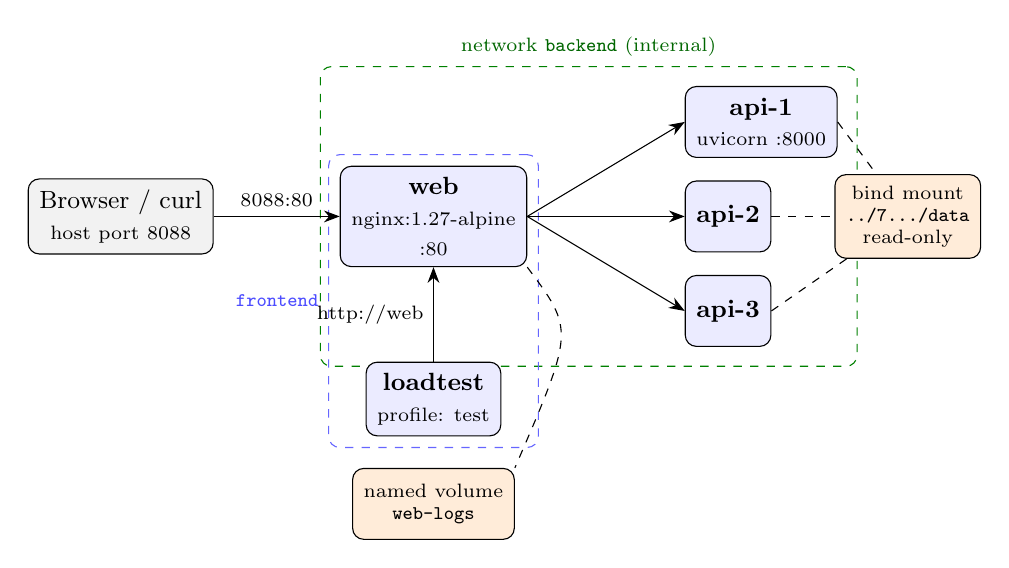
\begin{tikzpicture}[
  box/.style={draw,rounded corners,align=center,font=\small,minimum height=9mm,inner sep=4pt},
  svc/.style={box,fill=blue!8}, ext/.style={box,fill=gray!10}, vol/.style={box,fill=orange!15,font=\scriptsize},
  >={Stealth[length=2mm]}]
  \node[ext] (host) {Browser / curl\\\scriptsize host port 8088};
  \node[svc,right=16mm of host] (web) {\textbf{web}\\\scriptsize nginx:1.27-alpine\\\scriptsize :80};
  \node[svc,right=20mm of web,yshift=12mm] (a1) {\textbf{api-1}\\\scriptsize uvicorn :8000};
  \node[svc,right=20mm of web] (a2) {\textbf{api-2}};
  \node[svc,right=20mm of web,yshift=-12mm] (a3) {\textbf{api-3}};
  \node[svc,below=12mm of web] (lt) {\textbf{loadtest}\\\scriptsize profile: test};
  \node[vol,right=8mm of a2] (data) {bind mount\\\texttt{../7.../data}\\read-only};
  \node[vol,below=4mm of lt,xshift=0mm] (logs) {named volume\\\texttt{web-logs}};
  \draw[->] (host) -- node[above,font=\scriptsize]{8088:80} (web);
  \foreach \a in {a1,a2,a3} \draw[->] (web.east) -- (\a.west);
  \draw[->] (lt) -- node[left,font=\scriptsize]{http://web} (web);
  \draw[dashed] (a1.east) -- (data); \draw[dashed] (a2.east) -- (data); \draw[dashed] (a3.east) -- (data);
  \draw[dashed] (web.south east) .. controls +(0.6,-0.8) .. (logs.north east);
  \begin{scope}[on background layer]
    \node[draw=green!50!black,dashed,rounded corners,fit=(web)(a1)(a3),inner sep=7pt,
          label={[font=\scriptsize,green!40!black]above:network \texttt{backend} (internal)}] {};
    \node[draw=blue!60,dashed,rounded corners,fit=(web)(lt),inner sep=4pt,
          label={[font=\scriptsize,blue!70]left:\texttt{frontend}}] {};
  \end{scope}
\end{tikzpicture}
\caption{The stack. Only \texttt{web} has a host port. The api replicas sit on an internal network
with no route out, and nginx spreads requests over them.}
\label{fig:arch}
\end{figure}

% ---------------------------------------------------------------------------
\section{Docker design choices}

{\small
\begin{xltabular}{\linewidth}{@{}>{\raggedright\arraybackslash}p{3.3cm}L@{}}
\caption{Design choices and the reason for each}\\
\toprule
Choice & Reason \\
\midrule
\endfirsthead
\toprule
Choice & Reason \\
\midrule
\endhead
\multicolumn{2}{@{}l}{\textbf{Base images}} \\
\texttt{python:3.12-slim} (api, loadtest) & Debian-based, so the manylinux wheels of numpy, uvloop and httptools install
  without compiling. Alpine uses musl and would build numpy from source. Slim is about 4$\times$ smaller than the full
  \texttt{python} image. Python 3.12 is the version Lab 7 was tested with. \\
\texttt{nginx:1.27-alpine} (web) & nginx needs nothing from glibc. The image is 76\,MB and has \texttt{wget} for the
  healthcheck. It has an \texttt{envsubst} template step built in. \\
Two-stage api build & The builder stage creates a venv and installs the wheels. The runtime stage copies only
  \texttt{/opt/venv} and \texttt{app/}. Measured: 367\,MB (79.7\,MB compressed) against 422\,MB (107.7\,MB) for a naive one-stage
  Dockerfile (Figure~\ref{fig:size}). \\
Pinned tags & \texttt{nginx:1.27-alpine}, \texttt{python:3.12-slim}, and pinned versions in
  \texttt{requirements.txt}, so a rebuild next month gives the same stack. \\
\midrule
\multicolumn{2}{@{}l}{\textbf{Ports}} \\
\texttt{8088:80} on web only & The single entry point. The api replicas publish nothing (\texttt{EXPOSE 8000} is
  documentation only), so they cannot be reached from the host and cannot clash on a host port when scaled. 8080 was
  already taken on this laptop by Docker Desktop, so the host port is the variable \texttt{WEB\_PORT} (default 8088). \\
\midrule
\multicolumn{2}{@{}l}{\textbf{Networks}} \\
\texttt{frontend} (bridge) & web and loadtest. It is the side that faces clients. \\
\texttt{backend} (bridge, \texttt{internal: true}) & web and api. ``Internal'' means no gateway: the api has no
  route to the internet or the host (shown in Figure~\ref{fig:net}). The API needs no outbound access, so it gets
  none. \\
Docker DNS & Containers find each other by service name (\texttt{api}, \texttt{web}). nginx re-resolves
  \texttt{api} every 10\,s (\texttt{resolver 127.0.0.11 valid=10s}), so replicas added with \texttt{--scale} are used
  without restarting nginx. \\
\midrule
\multicolumn{2}{@{}l}{\textbf{Volumes}} \\
Bind mount \texttt{../7.Proximity\-SearchAPI/data} \texttt{:/data:ro} & The dataset (\texttt{locations.csv}, \texttt{link.txt})
  is data, not code. Mounting it means a new road file needs a restart, not a rebuild. \texttt{:ro} because the API
  only reads it. The image's build context excludes \texttt{data/}. \\
Named volume \texttt{web-logs} & nginx writes a copy of its access log there. It survives \texttt{docker compose
  down} and is removed only by \texttt{down -v} (Figure~\ref{fig:vol}). \\
\midrule
\multicolumn{2}{@{}l}{\textbf{Environment variables}} \\
\texttt{PORT}, \texttt{WORKERS} & uvicorn port and worker processes, read by the \texttt{CMD}. \texttt{API\_WORKERS} in
  \texttt{.env} sets them per run. \\
\texttt{LOCATIONS\_CSV}, \texttt{LINKS\_TXT} & Lab 7's loader already read these. They point it at \texttt{/data}. \\
\texttt{API\_UPSTREAM} & Turned into the nginx config by \texttt{envsubst} at start-up, so the proxy target is not
  hard-coded in the image. \\
\texttt{API\_REPLICAS}, \texttt{WEB\_PORT} & Compose-level variables (\texttt{deploy.replicas}, port mapping) with
  defaults 1 and 8088. \texttt{.env.example} lists them. \\
\texttt{PYTHON\-UNBUFFERED=1} & Python prints logs immediately, so \texttt{docker compose logs} shows them live. \\
\midrule
\multicolumn{2}{@{}l}{\textbf{Running safely}} \\
Non-root user & The api runs as \texttt{app} (uid 10001). Its packages are owned by root, so the process cannot
  change its own code or libraries. \\
Healthchecks & api: Python \texttt{urllib} GET of \texttt{/health} (slim has no curl). web: \texttt{wget} of
  \texttt{/nginx-health}. \texttt{depends\_on: condition: service\_healthy} starts nginx only after the API has loaded
  the graph. \\
\texttt{restart: unless-stopped} & A crashed process is restarted by Docker. A manual \texttt{docker stop} is
  respected. \\
\texttt{exec} in \texttt{CMD} & uvicorn becomes PID 1, so \texttt{docker stop}'s SIGTERM reaches it and it shuts down
  cleanly, instead of \texttt{sh} ignoring the signal until the 10\,s kill. \\
Per-Dockerfile \texttt{.docker\-ignore} & \texttt{api/Dockerfile.dockerignore} allows only \texttt{requirements.txt} and
  \texttt{app/}. The build context sent to Docker is 14\,kB, not the 3\,MB Lab 7 folder with its PDFs. \\
\bottomrule
\end{xltabular}}

% ---------------------------------------------------------------------------
\section{Steps followed}

All steps were run on the personal laptop, not on the allotted lab systems. Every figure in this
section is the real terminal output of that step, saved to \texttt{report/captures/*.txt} as it ran
and rendered as an image. Figure~\ref{fig:app} is a browser screenshot of the running stack.

\subsection{Install}
Docker Desktop for Mac (Apple silicon) was installed from docker.com. It bundles the engine, the
\texttt{docker} CLI and the Compose plugin, and runs the engine in a small Linux VM, which is why the
server reports \texttt{linux/arm64}. \texttt{hello-world} checks that the CLI can pull and run an image.
\shot{term_00_install.png}{0.85}{Install check: versions, the engine's VM, and \texttt{hello-world}.}

\subsection{Write the files}
\begin{center}\small
\begin{tabular}{ll}
\toprule
\texttt{api/Dockerfile}, \texttt{api/Dockerfile.dockerignore} & API image (two stages) \\
\texttt{web/Dockerfile}, \texttt{web/nginx.conf.template} & nginx image and its config \\
\texttt{loadtest/Dockerfile} & load-test client \\
\texttt{docker-compose.yml}, \texttt{.env.example} & the stack \\
\texttt{scripts/curl\_checks.sh}, \texttt{scripts/render\_terminal.py} & checks, and the figures in this report \\
\bottomrule
\end{tabular}
\end{center}
The full files are in Appendix~\ref{app:files}.

\subsection{Build}
\texttt{docker compose build} builds every service that has a \texttt{build:} section. With
\texttt{--no-cache} each step runs again; on this machine the three images took 16\,s, mostly
\texttt{pip install}. The build contexts are 68--261 bytes per step because of the ignore files.
\shot{term_01_build.png}{0.9}{Build: the stages of each image. \texttt{[api builder]} and \texttt{[api stage-1]} are
the two stages of the api image.}
\shot[fig:size]{term_01b_image_size.png}{0.9}{The two-stage api image against a one-stage version, and its layers. The runtime
image is the slim base plus the 128\,MB venv and the 53\,kB of code.}

\subsection{Run}
\texttt{docker compose up -d} creates the two networks, the volume, and the containers, in
dependency order. It waits until all three api replicas are healthy before starting web.
\shot{term_03_up.png}{0.9}{Run with three api replicas. Only \texttt{web} has a host port.}

\subsection{Verify}\label{sec:verify}
\shot{term_04_curl_through_nginx.png}{0.9}{The seven queries from the Lab 7 report, now through nginx. Results and
error messages match Lab 7 exactly, including \texttt{/search} without the trailing slash and the 400 errors.}
\shot[fig:app]{app_8088.png}{0.82}{Browser screenshot of \texttt{http://localhost:8088/}. The page is served by nginx, and its
\texttt{/network} and \texttt{/search/} calls go through nginx to an api replica.}
\shot{swagger_8088.png}{0.75}{FastAPI's \texttt{/docs} through the same proxy.}
\shot{term_02_tests_in_container.png}{0.9}{The 21 Lab 7 tests run inside the api image, with the Lab 7 folder mounted
read-only. This tests the code against the exact Python and library versions that run in production.}

\subsection{Scale and load}
nginx adds an \texttt{X-Upstream} header with the replica that answered. Nine requests reached all
three replicas, with no nginx restart after scaling. The 5{,}000-request load test runs in its own
container and reaches nginx at \texttt{http://web}.
\shot{term_05_scale.png}{0.9}{Requests spread over the three replicas (IPs match \texttt{docker inspect}).}
\shot{term_06_loadtest.png}{0.9}{Load test, 5{,}000 requests, 32 concurrent: 0 errors, about 890 req/s, p50 25\,ms. The
three replicas stay up after \texttt{compose run}, which was the fix for error 2 below.}

The load test is \emph{client-bound}. During the run the load-test container uses 98\,\% of one
CPU and each replica only about 10\,\%. Throughput was the same with one replica (884\,req/s) as with
three (889\,req/s). So these numbers measure the Python load generator, not the API. A faster client
(or several) would be needed to measure the API's limit. Lab 7 measured the search itself at
0.016\,ms per query.

\subsection{Networks, volumes, environment, restart}
\shot[fig:net]{term_07_networks.png}{0.9}{Network isolation. web reaches \texttt{api} by name; the api has no host port, cannot
resolve anything outside, and cannot even be resolved from the frontend network.}
\shot[fig:vol]{term_08_volumes.png}{0.9}{Volumes. The access log survives \texttt{compose down}/\texttt{up}. The dataset mount is
read-only, and the process runs as uid 10001.}
\shot{term_09_env.png}{0.9}{Environment variables inside the containers. With \texttt{API\_WORKERS=2} uvicorn runs as PID 1
with two worker processes.}
\shot{term_10_restart_logs.png}{0.9}{Self-healing. Sending SIGTERM to a replica's main process stops it, and Docker restarts
it (\texttt{RestartCount} 0$\to$1). In 600 requests sent while a replica restarted, all 600 returned 200, because
nginx retried the other replicas.}

\subsection{Tear down}
\texttt{docker compose down} removes containers and networks and keeps the \texttt{web-logs} volume.
\texttt{docker compose down -v} removes the volume too. \texttt{--rmi local} would also delete the three
built images.

% ---------------------------------------------------------------------------
\section{Errors faced and how they were resolved}

\paragraph{1. \texttt{pip install} in the api image: \emph{Permission denied}.}
To run the Lab 7 tests inside the image, pytest has to be installed into it first. As the default
user this failed:
\shot{term_err_01_pip_nonroot.png}{0.9}{Error 1.}
\emph{Cause:} the image runs as the non-root user \texttt{app}, and \texttt{/opt/venv} belongs to root,
which is the point of the non-root user. \emph{Fix:} the image was left as it is. The one-off test
container runs with \texttt{-u root}; the stack's own services never do. An alternative would be
a separate \texttt{test} stage in the Dockerfile with the dev dependencies.

\paragraph{2. \texttt{docker compose run} removed two of three replicas.}
After \texttt{docker compose up -d --scale api=3}, running the load test with
\texttt{docker compose run --rm loadtest} stopped and removed \texttt{api-4} and \texttt{api-5}:
\shot{term_err_02_run_resets_scale.png}{0.9}{Error 2: \texttt{run} brings dependencies back to their configured replica count.}
\emph{Cause:} \texttt{run} first makes sure the service's dependencies (web, and through web, api)
are running ``as configured''. The configuration said one api, and \texttt{--scale} on the earlier
command line was not part of it. The first time this appeared it was hidden by \texttt{run --build},
which also rebuilt the api image. \emph{Fix:} the number of replicas moved into the file,
\texttt{deploy.replicas: \$\{API\_REPLICAS:-1\}}, so every command sees the same desired state
(\texttt{API\_REPLICAS=3 docker compose up -d}). The loadtest image is built once with
\texttt{docker compose --profile test build loadtest}, then run without \texttt{--build}.

\paragraph{3. The log volume stored nothing.}
The \texttt{web-logs} volume was mounted at \texttt{/var/log/nginx}, but the directory only held two
links:
\shot{term_err_03_log_volume_symlinks.png}{0.9}{Error 3: the official nginx image links its log files to stdout and stderr.}
\emph{Cause:} the official image does this on purpose, so that \texttt{docker logs} works. When a new
named volume is mounted, Docker copies the image's directory into it, links included, so the log
still went to stdout and the volume was empty. \emph{Fix:} a second \texttt{access\_log} directive
writes to the file \texttt{proximity\_access.log} on the volume, while \texttt{access\_log /dev/stdout}
keeps \texttt{docker compose logs web} working (Figure~\ref{fig:vol}).

\paragraph{4. Port 8080 already in use.}
Before choosing the host port, \texttt{lsof -iTCP:8080 -sTCP:LISTEN} showed Docker Desktop already
listening there, and ports 3000, 3001, 8000 and 9090 belonged to another project's containers on the
same laptop. Publishing on 8080 would have failed with ``port is already allocated''. \emph{Fix:} the
host port is the variable \texttt{WEB\_PORT} with default 8088. A machine where 8088 is taken needs
only \texttt{WEB\_PORT=9000 docker compose up -d}.

% ---------------------------------------------------------------------------
\section{Docker commands}

\subsection{Commands used, in order}
\begin{lstlisting}[numbers=none]
docker version; docker compose version; docker info; docker run --rm hello-world
docker compose config -q                              # validate the compose file
docker compose --profile test build --no-cache        # build api, web, loadtest
docker images | grep proximity; docker history proximity-api:1.0
API_REPLICAS=3 docker compose up -d                   # start web + 3 api replicas
docker compose ps
scripts/curl_checks.sh                                # the Lab 7 queries through nginx
docker run --rm -u root -v "$PWD/../7.ProximitySearchAPI":/src:ro -w /src \
    proximity-api:1.0 sh -c "pip install -q pytest httpx; python -m pytest -q"
docker compose up -d --scale api=3
docker inspect -f '{{.Name}} {{range $k,$v := .NetworkSettings.Networks}}{{$k}}={{$v.IPAddress}} {{end}}' $(docker compose ps -q)
docker compose --profile test build loadtest
docker compose --profile test run --rm loadtest
docker stats --no-stream
docker network ls; docker network inspect proximity_backend
docker compose exec web wget -qO- http://api:8000/health
docker compose port api 8000
docker compose exec api python -c "import urllib.request; urllib.request.urlopen('https://pypi.org')"
docker compose --profile test run --rm --no-deps --entrypoint python loadtest -c "..."
docker volume ls
docker compose exec web tail -n 2 /var/log/nginx/proximity_access.log
docker compose down; docker compose up -d
docker compose exec api env; docker compose exec api id
API_WORKERS=2 docker compose up -d api
docker compose exec --index 1 api python -c "import os,signal; os.kill(1, signal.SIGTERM)"
docker inspect -f '{{.RestartCount}} {{.State.Health.Status}}' proximity-api-1
docker compose logs --tail 4 api
docker build -t proximity-api:single -f Dockerfile.single .   # size comparison only
docker rmi proximity-api:single
docker compose --profile test down -v
\end{lstlisting}

\subsection{Unique commands and their purpose}
\begin{table}[H]
\small
\begin{tabularx}{\linewidth}{@{}lL@{}}
\toprule
Command & Purpose \\
\midrule
\texttt{docker version} / \texttt{info} & client and engine versions; engine OS, CPUs, memory, storage driver \\
\texttt{docker run} & create and start a container from an image (\texttt{--rm} delete on exit, \texttt{-v} mount, \texttt{-u} user, \texttt{-w} working dir) \\
\texttt{docker build} & build an image from a Dockerfile and a context (\texttt{-t} tag, \texttt{-f} file) \\
\texttt{docker images} & list local images and their sizes \\
\texttt{docker history} & the layers of an image and the instruction that made each \\
\texttt{docker rmi} & delete an image \\
\texttt{docker inspect} & full JSON of a container, image, network or volume; \texttt{-f} picks fields with a Go template \\
\texttt{docker stats} & live CPU and memory per container (\texttt{--no-stream} one sample) \\
\texttt{docker network ls} / \texttt{inspect} & list networks; show subnet, \texttt{Internal}, attached containers \\
\texttt{docker volume ls} & list volumes \\
\midrule
\texttt{docker compose config} & merge the file with \texttt{.env} and print it; \texttt{-q} only validates \\
\texttt{docker compose build} & build every service with a \texttt{build:} section (\texttt{--no-cache}, \texttt{--profile}) \\
\texttt{docker compose up -d} & create networks, volumes and containers, start in dependency order, detached; \texttt{--build} rebuilds first, \texttt{--scale svc=N} sets replicas \\
\texttt{docker compose ps} & the stack's containers, status, health and ports \\
\texttt{docker compose run --rm} & one-off container for a service (here the load test); \texttt{--no-deps}, \texttt{--entrypoint} override \\
\texttt{docker compose exec} & run a command in a running service container; \texttt{--index} picks a replica \\
\texttt{docker compose logs} & the services' stdout and stderr (\texttt{--tail}, \texttt{-f}) \\
\texttt{docker compose port} & which host port a container port is published on \\
\texttt{docker compose down} & stop and remove containers and networks; \texttt{-v} also volumes, \texttt{--rmi} images \\
\midrule
\texttt{lsof -iTCP:8080 -sTCP:LISTEN} & (not Docker) which process already holds a host port \\
\bottomrule
\end{tabularx}
\end{table}

% ---------------------------------------------------------------------------
\section{What I learnt}

\begin{itemize}
  \item \textbf{An image is the code plus its exact runtime.} The Lab 7 tests passing inside the image
    means the API works with that Python, numpy and uvicorn, not only with whatever was on my laptop.
    On the lab systems in Lab 7 I had to ship wheels by hand because the boxes had no internet. An
    image solves that problem in one artifact.
  \item \textbf{Layers and their order matter.} Copying \texttt{requirements.txt} and installing before
    copying \texttt{app/} means a code change rebuilds only the last 53\,kB layer, not the 128\,MB of
    packages. A multi-stage build leaves build-only files behind; here that saved 55\,MB.
  \item \textbf{The build context is everything sent to the engine.} A per-Dockerfile ignore file cut
    it from the whole Lab 7 folder to 14\,kB, and kept the dataset out of the image.
  \item \textbf{Networks are a security boundary I can declare.} \texttt{internal: true} and publishing
    only nginx means the API is unreachable except through the proxy, and the API itself cannot
    reach out. Docker's DNS replaces hard-coded IPs, which is what makes \texttt{--scale} work.
  \item \textbf{Compose is desired state, not a list of commands.} Error 2 showed this clearly: a
    replica count given only on the command line was undone by the next command. Anything that should
    persist belongs in the file.
  \item \textbf{Data survives only where a volume is.} Containers are disposable: \texttt{down}
    deletes their filesystems. Named volumes and bind mounts are the only persistent parts, and an
    image's own setup (error 3) can make a volume silently useless.
  \item \textbf{Healthchecks turn ``started'' into ``ready''.} \texttt{depends\_on: service\_healthy}
    and the healthcheck together make nginx wait until the graph is loaded. A restart policy plus
    several replicas behind nginx meant a crashed replica cost zero failed requests.
  \item \textbf{Measure what you think you are measuring.} \texttt{docker stats} showed the load
    generator, not the API, was the bottleneck. Without it, 890\,req/s would have looked like the
    API's limit.
\end{itemize}

% ---------------------------------------------------------------------------
\appendix
\section{Files}\label{app:files}
\subsection*{\texttt{docker-compose.yml}}
\lstinputlisting[language=yaml]{../docker-compose.yml}
\subsection*{\texttt{api/Dockerfile}}
\lstinputlisting[language=docker]{../api/Dockerfile}
\subsection*{\texttt{web/Dockerfile}}
\lstinputlisting[language=docker]{../web/Dockerfile}
\subsection*{\texttt{web/nginx.conf.template}}
\lstinputlisting{../web/nginx.conf.template}
\subsection*{\texttt{loadtest/Dockerfile}}
\lstinputlisting[language=docker]{../loadtest/Dockerfile}
\subsection*{\texttt{api/Dockerfile.dockerignore}}
\lstinputlisting{../api/Dockerfile.dockerignore}

\end{document}
